% !TEX root = ../../../main.tex
\section{Cost and effort estimation: COCOMO II}
In this section we’re going to use COCOMO II approach to estimate the cost and effort needed for developing PowerEnJoy system.

\subsection{Scale Drivers}
For estimating scale drivers values we refer to the official COCOMO II table:

\begin{table}[H]
	\begin{adjustwidth}{-.5in}{-.5in}
		\caption[Scale Drivers values]{Scale Drivers values for COCOMO II Model}
		\label{table:scale_drivers}
		\begin{tabularx}{1.25\textwidth}{| X | X | X | X | X | X | X |}
			\hline
			Scale Factors	&	Very Low	&	Low	&	Nominal	&	High	&	Very High	&	Extra High \\ \hline
			
			PREC	&	thoroughly unprecedented	&	\textbf{largely unprecedented}	&	somewhat unprecedented	&	generally familiar	&	largely familiar	&	thoroughly familiar \\
			SF\textsubscript{j}	&	6.20	&	\textbf{4.96}	&	3.72	&	2.48	&	1.24	&	0.00 \\ \hline
			
			FLEX	&	rigorous	&	\textbf{occasional relaxation}	&	some relaxation	&	general conformity	&	some conformity	&	general goals \\
			SF\textsubscript{j}	&	5.07	&	\textbf{4.05}	&	3.04	&	2.03	&	1.01	&	0.00 \\ \hline
			
			RESL	&	little (20\%)	&	some (40\%)	&	often (60\%)	&	generally (75\%)	&	\textbf{mostly (90\%)	}&	full (100\%) \\
			SF\textsubscript{j}	&	7.07	&	5.65	&	4.24	&	2.83	&	\textbf{1.41}	&	0.00 \\ \hline
			
			TEAM	&	very difficult interactions	&	some difficult interactions	&	basically cooperative interactions	&	largely cooperative	&	\textbf{highly cooperative}	&	seamless interactions \\
			SF\textsubscript{j}	&	5.48	&	4.38&	3.29	&	2.19	&	\textbf{1.10}	&	0.00 \\ \hline
			
			PMAT	&	SW-CMM Level 1 Lower	&	SW-CMM Level 1 Upper	&	SW-CMM Level 2	&	\textbf{SW-CMM Level 3}	&	SW-CMM Level 4	&	SW-CMM Level 5 \\
			SF\textsubscript{j}	&	7.80	&	6.24	&	4.68	&	\textbf{3.12}	&	1.56	&	0.00 \\ \hline
		\end{tabularx}
	\end{adjustwidth}
\end{table}

Here a brief description of scale drivers considered above:
\begin{itemize}
	\item Precedentedness - It reflects the previous experience of the team with the development of similar projects.
	
\begin{table}[H]
	\centering
	\caption{PREC Rating Levels}
	\label{tab:prec_rating_levels}
	\begin{adjustwidth}{-.5in}{-.5in}
	\begin{tabularx}{1.25\textwidth}{|>{\hsize=.4\hsize}X|>{\centering\arraybackslash\hsize=.2\hsize}X|>{\centering\arraybackslash\hsize=.2\hsize}X|>{\centering\arraybackslash\hsize=.2\hsize}X|}
		\hline
		Feature		&	Very Low	&	Nominal / High	&	Extra High \\ \hline
		Organizational understanding of product objectives	&	General	&	\textbf{Considerable}	&	Thorough	\\ \hline
		Experience in working with related software systems	&	\textbf{Moderate}	&	Considerable	&	Extensive	\\ \hline
		Concurrent development of associated new hardware and operational procedures	&	\textbf{Extensive}	&	Moderate	&	Some	\\ \hline
		Need for innovative data processing architectures, algorithms	&	Considerable	&	\textbf{Some}	&	Minimal	\\ \hline
	\end{tabularx}
	\end{adjustwidth}
\end{table}	
	
	\item Development Flexibility -  It reflects the degree of flexibility in the development process with respect to specific constraints, requirements and external specifications.
	
\begin{table}[H]
	\centering
	\caption{FLEX Rating Levels}
	\label{tab:flex_rating_levels}
	\begin{adjustwidth}{-.5in}{-.5in}
	\begin{tabularx}{1.25\textwidth}{|>{\hsize=.4\hsize}X|>{\centering\arraybackslash\hsize=.2\hsize}X|>{\centering\arraybackslash\hsize=.2\hsize}X|>{\centering\arraybackslash\hsize=.2\hsize}X|}
		\hline
		Feature		&	Very Low	&	Nominal / High	&	Extra High \\ \hline
		
		Need for software conformance with pre-established requirements	&	\textbf{Full}	&	Considerable	&	Basic	\\ \hline
		
		Need for software conformance with external interface specifications	&	Full	&	\textbf{Considerable}	&	Basic	\\ \hline
		
		Combination of inflexibilities above with premium on early completion	&	High	&	\textbf{Medium}	&	Low	\\ \hline
	\end{tabularx}
	\end{adjustwidth}
\end{table}	
	
	\item Risk Resolution - It reflects the level of analysis with respect to the risk management plan and the definition of budget and schedule.
	
\begin{table}[H]
	\centering
	\caption{RESL Rating Levels}
	\label{tab:resl_rating_levels}
	\begin{adjustwidth}{-.5in}{-.5in}
	\begin{tabularx}{1.25\textwidth}{|>{\hsize=.25\hsize}X|>{\centering\arraybackslash\hsize=.125\hsize}X|>{\centering\arraybackslash\hsize=.125\hsize}X|>{\centering\arraybackslash\hsize=.125\hsize}X|>{\centering\arraybackslash\hsize=.125\hsize}X|>{\centering\arraybackslash\hsize=.125\hsize}X|>{\centering\arraybackslash\hsize=.125\hsize}X|}
		\hline
		Characteristic		&	Very Low	&	Low	&	Nominal	&	High	&	Very High	&	Extra High\\ \hline
		
		Risk Management Plan identifies all critical risk items, establishes milestones for resolving them by PDR or LCA.	&	None	&	Little	&	Some	&	Generally	&	\textbf{Mostly}	&	Fully	\\ \hline	
		Schedule, budget, and internal milestones through PDR or LCA compatible with Risk Management Plan.	&	None	&	Little	&	Some	&	\textbf{Generally}	&	Mostly	&	Fully	\\ \hline
%		
		Percent of development schedule devoted to establishing architecture, given general product objectives.	&	5	&	10	&	17	&	\textbf{25}	&	33	&	40\\ \hline
		
		Percent of required top software architects available to project.	&	20	&	40	&	60	&	80	&	\textbf{100}	&	120\\ \hline
		
		Tool support available for resolving risk items, developing and verifying architectural specs.	&	None	&	Little	&	Some	&	Good	&	\textbf{Strong}	&	Full\\ \hline
		
		Level of uncertainty in key architecture drivers: mission, user interface, COTS, hardware, technology, performance.	&	Extreme	&	Significant	&	Consider- able	&	Some	&	\textbf{Little}	&	Very Little\\ \hline
		
		Number and criticality of risk items.	&	$>$ 10 Critical	&	5-10 Critical	&	\textbf{2-4 Critical}	&	1 Critical	&	$>$ 5 Non Critical	&	$<$ 5 Non Critical\\ \hline
	\end{tabularx}
	\end{adjustwidth}
\end{table}	
	
	\item Team Cohesion - It reflects the level of coordination and synchronization of project's stakholders: users, customers, developers, maintainers, interfacers, others.
	
\begin{table}[H]
	\centering
	\caption{TEAM Rating Levels}
	\label{tab:team_rating_levels}
	\begin{adjustwidth}{-.5in}{-.5in}
	\begin{tabularx}{1.25\textwidth}{|>{\hsize=.25\hsize}X|>{\centering\arraybackslash\hsize=.125\hsize}X|>{\centering\arraybackslash\hsize=.125\hsize}X|>{\centering\arraybackslash\hsize=.125\hsize}X|>{\centering\arraybackslash\hsize=.125\hsize}X|>{\centering\arraybackslash\hsize=.125\hsize}X|>{\centering\arraybackslash\hsize=.125\hsize}X|}
		\hline
		Characteristic		&	Very Low	&	Low	&	Nominal	&	High	&	Very High	&	Extra High\\ \hline
		
		Consistency of stakeholder objectives and cultures	&	Little	&	Some	&	Basic	&	Consider- able	&	Strong	&	\textbf{Full}	\\ \hline	
		
		Ability, willingness of stakeholders to accommodate other stakeholders? objectives	&	Little	&	Some	&	Basic	&	Consider- able	&	\textbf{Strong}	 &	Full	\\ \hline	
%		
		Experience of stakeholders in operating as a team	&	None	&	Little	&	Little	&	Basic	&	Consider- able	&	\textbf{Extensive}\\ \hline
		
		Stakeholder teambuilding to achieve shared vision and commitments	&	None	&	Little	&	Little	&	Basic	&	Consider- able	&	\textbf{Extensive} \\
		\hline
	\end{tabularx}
	\end{adjustwidth}
\end{table}	
	
	\item Process Maturity - It reflects the level of maturity of the software organization.
\end{itemize}

\begin{figure}[H]
	\centering
	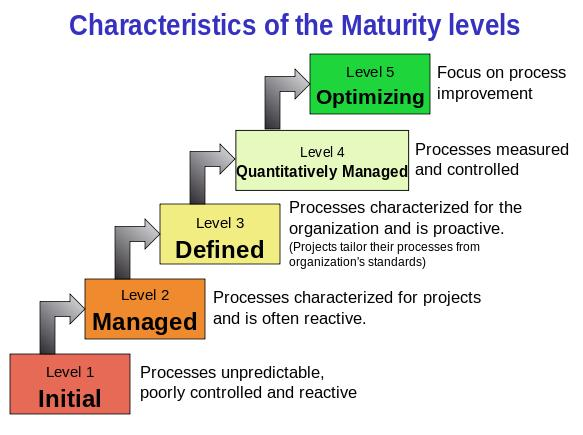
\includegraphics[width=0.7\textwidth]{CMM-levels}
	\caption[CMM Levels]{The picture above shows levels of process maturity defined by SW-CMM.}
	\label{fig:CMM-Levels}
\end{figure}

Here the result of scale drivers' evaluation:

\begin{table}[H]
	\centering
	\caption{Scale Drivers overall estimation}
	\label{tab:overall_sd}
	\begin{tabular}{|l|l|l|}
		\hline
		Scale Driver		&	Factor	&	Value	\\ \hline
		Precedentedness (PREC)			&	Low			&	4.96	\\
		Development flexibility (FLEX)	&	Low			&	4.05	\\ 
		Risk resolution (RESL)			&	Very high	&   1.41	\\
		Team cohesion (TEAM)			&   Very high   &   1.10	\\
		Process maturity (PMAT)			&	Level 3		&	3.12	\\ \hline
		\multicolumn{2}{| l |}{Total}					&	14.64\\
		\hline
	\end{tabular}
\end{table}

\subsection{Cost Drivers}

\subsubsection{Required Software Reliability}
This is the measure of the extent to which the software must perform its intended function over a period of time. Supposing that electric car sharing will be largely used in the near future and the system will have great success, a potential malfunctioning could lead to high financial losses.

\begin{table}[H]
	\begin{adjustwidth}{-.5in}{-.5in}
		\caption{RELY values}
		\label{table:rely}
		\begin{tabularx}{1.25\textwidth}{| X | X | X | X | X | X | X |}
			\hline
			\multicolumn{7}{| c |}{RELY Cost Drivers}	\\ \hhline{|=======|}
			RELY Descriptors	&	slightly inconvinience	&	easily recoverable losses	&	moderate recoverabile losses	&	high financial loss	&	risk to human life	&	 \\ \hline
			
			Rating level	&	Very Low	&	Low	&	Nominal	&	\textbf{High}	&	Very High	&	Extra High \\ \hline
			Effort multipliers	&	0.82	&	0.92	&	1.00	&	\textbf{1.10}	&	1.26	&	n/a \\ \hline
		\end{tabularx}
	\end{adjustwidth}
\end{table}

\subsubsection{Database Size}
This cost driver attempts to capture the effect large test data requirements have on product development. The rating is determined by calculating D/P, the ratio of bytes in the testing database to SLOC in the program. The reason the size of the database is important to consider is because of the effort required to generate the test data that will be used to exercise the program. In the case of PowerEnJoy a 5 Mb testing database has been estimated and for this reason:
\begin{center}
	$\frac{D}{P} = 5*10^6 / 6042 = 828$
\end{center}

\begin{table}[H]
	\begin{adjustwidth}{-.5in}{-.5in}
		\caption{DATA values}
		\label{table:data}
		\begin{tabularx}{1.25\textwidth}{| X | X | X | X | X | X | X |}
			\hline
			\multicolumn{7}{| c |}{DATA Cost Drivers}	\\ \hhline{|=======|}
			DATA Descriptors	&	&	$\frac{D}{P}$ \textless\! 10	&	10 \!\textless\! $\frac{D}{P}$ \textless\! 100	&	100 \!\textless\! $\frac{D}{P}$ \textless\! 1000	&	$\frac{D}{P}$ \textgreater\! 1000	&	 \\ \hline
			
			Rating level	&	Very Low	&	Low	&	Nominal	&	High	&	Very High	&	Extra High \\ \hline
			Effort multipliers	&	n/a	&	0.90	&	1.00	&	\textbf{1.14}	&	1.28	&	n/a \\ \hline
		\end{tabularx}
	\end{adjustwidth}
\end{table}

\subsubsection{Product Complexity}
According to COCOMO II rating scale, the complexity of development of the system is considered high.

\begin{table}[H]
	\begin{adjustwidth}{-.5in}{-.5in}
		\caption{CPLX values}
		\label{table:cplx}
		\begin{tabularx}{1.25\textwidth}{| X | X | X | X | X | X | X |}
			\hline
			\multicolumn{7}{| c |}{CPLX Cost Drivers}	\\ \hhline{|=======|}
			Rating level	&	Very Low	&	Low	&	Nominal	&	\textbf{High}	&	Very High	&	Extra High \\ \hline
			Effort multipliers	&	0.73	&	0.87	&	1.00	&	\textbf{1.17}	&	1.34	&	1.74 \\ \hline
		\end{tabularx}
	\end{adjustwidth}
\end{table}

\subsubsection{Required Reusability}
This cost driver accounts for the additional effort needed to construct components intended for reuse on current or future projects. “Across program” could apply to reuse across multiple financial applications projects for a single organization: for example some system's components could be reused for other "sharing-systems".

\begin{table}[H]
	\begin{adjustwidth}{-.5in}{-.5in}
		\caption{RUSE values}
		\label{table:ruse}
		\begin{tabularx}{1.25\textwidth}{| X | X | X | X | X | X | X |}
			\hline
			\multicolumn{7}{| c |}{RUSE Cost Drivers}	\\ \hhline{|=======|}
			RUSE Descriptors	&	&	None	&	Across project	&	Across program	&	Across product line	&	Across multiple product lines \\ \hline
			Rating level	&	Very Low	&	Low	&	Nominal	&	\textbf{High}	&	Very High	&	Extra High \\ \hline
			Effort multipliers	&	n/a	&	0.95	&	1.00	&	\textbf{1.07}	&	{1.15}	&	1.24 \\ \hline
		\end{tabularx}
	\end{adjustwidth}
\end{table}

\subsubsection{Documentation match to life-cycle needs}
The rating scale for the DOCU cost driver is evaluated in terms of the suitability of the project’s documentation to its life-cycle needs.

\begin{table}[H]
	\begin{adjustwidth}{-.5in}{-.5in}
		\caption{DOCU values}
		\label{table:docu}
		\begin{tabularx}{1.25\textwidth}{| X | X | X | X | X | X | X |}
			\hline
			\multicolumn{7}{| c |}{DOCU Cost Drivers}	\\ \hhline{|=======|}
			DOCU Descriptors	&	Many life-cycle needs uncovered	&	Some life-cycle needs uncovered	&	Right-sized to life-cycle needs	&	Excessive for life- cycle needs	&	Very excessive for life-cycle needs	&	 \\ \hline
			Rating level	&	Very Low	&	Low	&	\textbf{Nominal}	&	High	&	Very High	&	Extra High \\ \hline
			Effort multipliers	&	0.81	&	0.91	&	\textbf{1.00}	&	1.11	&	1.23	&	n/a \\ \hline
		\end{tabularx}
	\end{adjustwidth}
\end{table}

\subsubsection{Execution Time Constraint}
This is a measure of the execution time constraint imposed upon a software system. The
rating is expressed in terms of the percentage of available execution time expected to be used by
the system or subsystem consuming the execution time resource.

\begin{table}[H]
	\begin{adjustwidth}{-.5in}{-.5in}
		\caption{TIME values}
		\label{table:time}
		\begin{tabularx}{1.25\textwidth}{| X | X | X | X | X | X | X |}
			\hline
			\multicolumn{7}{| c |}{TIME Cost Drivers}	\\ \hhline{|=======|}
			TIME Descriptors	&	&	&	$\leq$ 50\% use of available execution time	&	70\% use of available execution time	&	85\% use of available execution time	&	95\% use of available execution time \\ \hline
			Rating level	&	Very Low	&	Low	&	Nominal	&	\textbf{High}	&	Very High	&	Extra High \\ \hline
			Effort multipliers	&	n/a	&	n/a	&	1.00	&	\textbf{1.11}	&	1.29	&	1.63 \\ \hline
		\end{tabularx}
	\end{adjustwidth}
\end{table}

\subsubsection{Storage Constraint}
This rating represents the degree of main storage constraint imposed on a software system or subsystem. 

\begin{table}[H]
	\begin{adjustwidth}{-.5in}{-.5in}
		\caption{STOR values}
		\label{table:stor}
		\begin{tabularx}{1.25\textwidth}{| X | X | X | X | X | X | X |}
			\hline
			\multicolumn{7}{| c |}{STOR Cost Drivers}	\\ \hhline{|=======|}
			STOR Descriptors	&	&	&	$\leq$ 50\% use of available storage	&	70\% use of available storage	&	85\% use of available storage	&	95\% use of available storage \\ \hline
			Rating level	&	Very Low	&	Low	&	\textbf{Nominal}	&	High	&	Very High	&	Extra High \\ \hline
			Effort multipliers	&	n/a	&	n/a	&	\textbf{1.00}	&	1.05	&	1.17	&	1.46 \\ \hline
		\end{tabularx}
	\end{adjustwidth}
\end{table}

\subsubsection{Platform Volatility}
“Platform” is used here to mean the complex of hardware and software the software product calls on to perform its tasks; the platform includes any compilers or assemblers supporting the development of the software system. We estimate that a major release of the software will be needed about every 12 months.

\begin{table}[H]
	\begin{adjustwidth}{-.5in}{-.5in}
		\caption{PVOL values}
		\label{table:pvol}
		\begin{tabularx}{1.25\textwidth}{| X | X | X | X | X | X | X |}
			\hline
			\multicolumn{7}{| c |}{PVOL Cost Drivers}	\\ \hhline{|=======|}
			PVOL Descriptors	&	&	Major change every 12 mo., minor change every 1 mo.	&	Major: 6mo; minor: 2wk.	&	Major: 2mo, minor: 1wk	&	Major: 2wk; mi- nor: 2 days	&	 \\ \hline
			Rating level	&	Very Low	&	\textbf{Low}	&	Nominal	&	High	&	Very High	&	Extra High \\ \hline
			Effort multipliers	&	n/a	&	\textbf{0.87}	&	1.00	&	1.15	&	1.30	&	n/a \\ \hline
		\end{tabularx}
	\end{adjustwidth}
\end{table}

\subsubsection{Analyst Capability}
Analysts are personnel who work on requirements, high-level design and detailed design. The major attributes that should be considered in this rating are analysis and design ability, efficiency and thoroughness, and the ability to communicate and cooperate.

\begin{table}[H]
	\begin{adjustwidth}{-.5in}{-.5in}
		\caption{ACAP values}
		\label{table:acap}
		\begin{tabularx}{1.25\textwidth}{| X | X | X | X | X | X | X |}
			\hline
			\multicolumn{7}{| c |}{ACAP Cost Drivers}	\\ \hhline{|=======|}
			ACAP Descriptors	&	15th percentile	&	35th percentile	&	55th percentile	&	75th percentile	&	90th percentile	&	 \\ \hline
			Rating level	&	Very Low	&	Low	&	Nominal	&	\textbf{High}	&	Very High	&	Extra High \\ \hline
			Effort multipliers	&	1.42	&	1.19	&	1.00	&	\textbf{0.85}	&	0.71	&	n/a \\ \hline
		\end{tabularx}
	\end{adjustwidth}
\end{table}

\subsubsection{Programmer Capability}
Evaluation for this cost driver should be based on the capability of the programmers as a team rather than as individuals. Major factors which should be considered in the rating are ability, efficiency and thoroughness, and the ability to communicate and cooperate.

\begin{table}[H]
	\begin{adjustwidth}{-.5in}{-.5in}
		\caption{PCAP values}
		\label{table:pcap}
		\begin{tabularx}{1.25\textwidth}{| X | X | X | X | X | X | X |}
			\hline
			\multicolumn{7}{| c |}{PCAP Cost Drivers}	\\ \hhline{|=======|}
			PCAP Descriptors	&	15th percentile	&	35th percentile	&	55th percentile	&	75th percentile	&	90th percentile	&	 \\ \hline
			Rating level	&	Very Low	&	Low	&	\textbf{Nominal}	&	High	&	Very High	&	Extra High \\ \hline
			Effort multipliers	&	1.34	&	1.15	&	\textbf{1.00}	&	0.88	&	0.76	&	n/a \\ \hline
		\end{tabularx}
	\end{adjustwidth}
\end{table}

\subsubsection{Application Experience}
The rating for this cost driver is dependent on the level of applications experience of the project team developing the software system or subsystem. The ratings are defined in terms of the project team’s equivalent level of experience with this type of application.

\begin{table}[H]
	\begin{adjustwidth}{-.5in}{-.5in}
		\caption{APEX values}
		\label{table:apex}
		\begin{tabularx}{1.25\textwidth}{| X | X | X | X | X | X | X |}
			\hline
			\multicolumn{7}{| c |}{APEX Cost Drivers}	\\ \hhline{|=======|}
			APEX Descriptors	&	$\leq$ 2 months	&	6 months	&	1 year	&	3 years	&	6 years	&	 \\ \hline
			Rating level	&	\textbf{Very Low}	&	Low	&	Nominal	&	High	&	Very High	&	Extra High \\ \hline
			Effort multipliers	&	\textbf{1.22}	&	1.10	&	1.00	&	0.88	&	0.81	&	n/a \\ \hline
		\end{tabularx}
	\end{adjustwidth}
\end{table}

\subsubsection{Platform Experience}
The Post-Architecture model broadens the productivity influence of platform experience by recognizing the importance of understanding the use of more powerful platforms, including more graphic user interface, database, networking, and distributed middleware capabilities.

\begin{table}[H]
	\begin{adjustwidth}{-.5in}{-.5in}
		\caption{PLEX values}
		\label{table:plex}
		\begin{tabularx}{1.25\textwidth}{| X | X | X | X | X | X | X |}
			\hline
			\multicolumn{7}{| c |}{PLEX Cost Drivers}	\\ \hhline{|=======|}
			PLEX Descriptors	&	$\leq$ 2 months	&	6 months	&	1 year	&	3 years	&	6 years	&	 \\ \hline
			Rating level	&	Very Low	&	\textbf{Low}	&	Nominal	&	High	&	Very High	&	Extra High \\ \hline
			Effort multipliers	&	1.19	&	\textbf{1.09}	&	1.00	&	0.91	&	0.85	&	n/a \\ \hline
		\end{tabularx}
	\end{adjustwidth}
\end{table}

\subsubsection{Language and Tool Experience}
This is a measure of the level of programming language and software tool experience of the project team developing the software system or subsystem. In addition to experience in the project’s programming language, experience on the project’s supporting tool set also affects development effort.

\begin{table}[H]
	\begin{adjustwidth}{-.5in}{-.5in}
		\caption{LTEX values}
		\label{table:ltex}
		\begin{tabularx}{1.25\textwidth}{| X | X | X | X | X | X | X |}
			\hline
			\multicolumn{7}{| c |}{LTEX Cost Drivers}	\\ \hhline{|=======|}
			LTEX Descriptors	&	$\leq$ 2 months	&	6 months	&	1 year	&	3 years	&	6 years	&	 \\ \hline
			Rating level	&	Very Low	&	Low	&	\textbf{Nominal}	&	High	&	Very High	&	Extra High \\ \hline
			Effort multipliers	&	1.20	&	1.09	&	\textbf{1.00}	&	0.91	&	0.84	&	n/a \\ \hline
		\end{tabularx}
	\end{adjustwidth}
\end{table}

\subsubsection{Personnel Continuity}
The rating scale for PCON is in terms of the project’s annual personnel turnover: team members have been the same since the begin until the end of development.

\begin{table}[H]
	\begin{adjustwidth}{-.5in}{-.5in}
		\caption{PCON values}
		\label{table:pcon}
		\begin{tabularx}{1.25\textwidth}{| X | X | X | X | X | X | X |}
			\hline
			\multicolumn{7}{| c |}{PCON Cost Drivers}	\\ \hhline{|=======|}
			PCON Descriptors	&	48\% / year	&	24\% / year	&	12\% / year	&	6\% / year	&	3\% / year	&	 \\ \hline
			Rating level	&	Very Low	&	Low	&	Nominal	&	High	&	\textbf{Very High}	&	Extra High \\ \hline
			Effort multipliers	&	1.29	&	1.12	&	1.00	&	0.90	&	\textbf{0.81}	&	n/a \\ \hline
		\end{tabularx}
	\end{adjustwidth}
\end{table}

\subsubsection{Usage of Software Tools}
The tool rating ranges from simple edit and code, very low, to integrated life-cycle management tools, very high.

\begin{table}[H]
	\begin{adjustwidth}{-.5in}{-.5in}
		\caption{TOOL values}
		\label{table:tool}
		\begin{tabularx}{1.25\textwidth}{| X | X | X | X | X | X | X |}
			\hline
			\multicolumn{7}{| c |}{TOOL Cost Drivers}	\\ \hhline{|=======|}
			TOOL Descriptors	&	edit, code, debug	&	simple, frontend, backend CASE, little integration	&	basic life-cycle tools, moderately integrated	&	strong, mature life-cycle tools, moderately integrated	&	strong, mature, proactive life-cycle tools, well integrated with processes, methods, reuse	&	 \\ \hline
			Rating level	&	Very Low	&	Low	&	Nominal	&	\textbf{High}	&	Very High	&	Extra High \\ \hline
			Effort multipliers	&	1.17	&	1.09	&	1.00	&	\textbf{0.90}	&	0.78	&	n/a \\ \hline
		\end{tabularx}
	\end{adjustwidth}
\end{table}

\subsubsection{Multisite Development}
Determining its cost driver rating involves the assessment and judgement-based averaging of two factors: site collocation (from fully collocated to international distribution) and communication support (from surface mail and some phone access to full interactive multimedia).

\begin{table}[H]
	\begin{adjustwidth}{-.5in}{-.5in}
		\caption{SITE values}
		\label{table:site}
		\begin{tabularx}{1.25\textwidth}{| X | X | X | X | X | X | X |}
			\hline
			\multicolumn{7}{| c |}{SITE Cost Drivers}	\\ \hhline{|=======|}
			SITE Collocation Descriptors	&	Inter- national	&	Multi-city and multi-company	&	Multi-city or multi-company	&	Same city or metro area	&	Same building or complex	&	Fully collocated \\
			SITE Communications Descriptors	&	Some phone, mail	&	Individual phone, fax	&	
Narrow band email	&	Wideband electronic communication	&	Wideband elect. comm., occasional video conf.	&	Interactive multimedia \\ \hline
			Rating level	&	Very Low	&	Low	&	Nominal	&	\textbf{High}	&	Very High	&	Extra High \\ \hline
			Effort multipliers	&	1.22	&	1.09	&	1.00	&	\textbf{0.93}	&	0.86	&	0.80 \\ \hline
		\end{tabularx}
	\end{adjustwidth}
\end{table}

\subsubsection{Required Development Schedule}
This rating measures the schedule constraint imposed on the project team developing the software. The ratings are defined in terms of the percentage of schedule stretch-out or acceleration with respect to a nominal schedule for a project requiring a given amount of effort. Accelerated schedules tend to produce more effort in the earlier phases to eliminate risks and refine the architecture, more effort in the later phases to accomplish more testing and documentation in parallel.

\begin{table}[H]
	\begin{adjustwidth}{-.5in}{-.5in}
		\caption{SCED values}
		\label{table:sced}
		\begin{tabularx}{1.25\textwidth}{| X | X | X | X | X | X | X |}
			\hline
			\multicolumn{7}{| c |}{SCED Cost Drivers}	\\ \hhline{|=======|}
			SCED Descriptors	&	75\% of nominal	&	85\% of nominal	&	100\% of nominal	&	130\% of nominal	&	160\% of nominal	&	 \\ \hline
			Rating level	&	Very Low	&	Low	&	\textbf{Nominal}	&	High	&	Very High	&	Extra High \\ \hline
			Effort multipliers	&	1.43	&	1.14	&	\textbf{1.00}	&	1.00	&	1.00	&	n/a \\ \hline
		\end{tabularx}
	\end{adjustwidth}
\end{table}


\subsubsection{Cost Driver overall estimation}
Here the result of cost drivers' evaluation:

\begin{table}[H]
	\centering
	\caption{Cost Drivers overall estimation}
	\label{tab:overall_cd}
	\begin{tabular}{|l|l|l|}
		\hline
		Cost Driver		&	Factor	&	Value	\\ \hline
		Required Software Reliability (RELY)			&	High		&	1.10	\\
		Database size (DATA)							&	High		&	1.14	\\
		Product complexity (CPLX)						&	High		&	1.17	\\
		Required Reusability (RUSE)						&	High		&	1.07	\\
		Documentation match to life-cycle needs (DOCU)	&	Nominal		&	1.00	\\
		Execution Time Constraint (TIME)				&	High		&	1.11	\\
		Main storage constraint (STOR)					&	Nominal		&	1.00	\\
		Platform volatility (PVOL)						&	Low			&	0.87	\\
		Analyst capability (ACAP)						&	High		&	0.85	\\
		Programmer capability (PCAP)					&	Nominal		&	1.00	\\
		Application Experience (APEX)					&	Very low	&	1.22	\\
		Platform Experience (PLEX)						&	Low			&	1.09	\\
		Language and Tool Experience (LTEX)				&	Nominal		&	1.00	\\
		Personnel continuity (PCON)						&	Very high	&	0.81	\\
		Usage of Software Tools (TOOL)					&	High		&	0.90	\\
		Multisite development (SITE)					&	High		&	0.93	\\
		Required development schedule (SCED)			&	Nominal		&	1.00	\\	\hline
		\multicolumn{2}{| l |}{Total (EAF)}									&	1.1618\\
		\hline
	\end{tabular}
\end{table}

\subsection{Effort Equation}
COCOMO II provides the following equation to estimate the effort required measured in Person-Months (PM):
\begin{center}
$Effort = A * EAF * KSLOC^E$
\end{center}
Where:
\begin{itemize}
	\item $A$ is a constant that approximates the productivity in PM / KSLOC
	\item $EAF$ is the product of all the effort multipliers derived from the Cost Drivers
	\item $E$ is an aggregation of the five Scale Factors obtained with the following equation:
	\begin{center}
		$E = B + 0.01 * \sum\limits_{j=1}^5 SF_j$
	\end{center}
	where $B = 0.91$.
\end{itemize}
Given that,
\begin{center}
$A = 2.94$ \\[10pt]
$E = B + 0.01 * 14.64 = 1.0564$ \\[10pt]
$EAF = \prod\limits_{i=1}^{15} EM_i = 1.1618$
\end{center}
the $Effort$ can be calculated as:
\begin{center}
$Effort = 2.94 * 1.1618 * 6.042^{1.0564} = 22.8411 PM \simeq 23 PM$
\end{center}

\subsection{Schedule Estimation}
COCOMO II provides also an equation to estimate the project duration given the parameter previously calculated:
\begin{center}
	$Duration = 3.67 * Effort^F$
\end{center}
where $F$ is equal to:
\begin{center}
	$F = 0.28 + 0.2 * (E - B)$
\end{center}
Given that,
\begin{center}
	$F = 0.28 + 0.2 * (1.0564 - 0.91) = 0.3093$ \\[10pt]
	$Effort = 22.8411 PM$
\end{center}
the $Duration$ can be calculated as:
\begin{center}
	$Duration = 3.67 * 22.8411^{0.3093} = 9.66 \ months$
\end{center}
